\documentclass[a4paper,10pt]{article}
\usepackage[margin=1in]{geometry}
\usepackage{amsmath,amsthm,amssymb,amsfonts,stmaryrd}
\usepackage{soul}
\usepackage{array}
\usepackage{empheq}
\usepackage{xfrac}
\usepackage{minibox}
\usepackage{enumitem}
	\setlist{nosep} % or \setlist{noitemsep} to leave space around whole list
\usepackage{color}
\usepackage{blkarray}
\setcounter{MaxMatrixCols}{20}
\usepackage{showlabels}
\usepackage{arydshln}	% Dotted lines in arrays
\usepackage{adjustbox}
\usepackage{hyperref}
\hypersetup{
  colorlinks   = true, %Colours links instead of ugly boxes
  urlcolor     = blue, %Colour for external hyperlinks
  linkcolor    = blue, %Colour of internal links
  citecolor   = red %Colour of citations
}
\usepackage{cleveref}


\newtheorem{lemma}{Lemma}
\newtheorem{definition}{Definition}
\newtheorem{theorem}{Theorem}
\newtheorem{corollary}{Corollary}

\newcommand{\tcb}{\textcolor{blue}}
\newcommand{\todo}[1]{\textcolor{red}{[TODO\@: #1]}}


\begin{document}
\allowdisplaybreaks

% ---------------------------------------------------------------------------------------------- %
% ---------------------------------------------------------------------------------------------- %
% ---------------------------------------------------------------------------------------------- %
\section{Eigenvalue analysis}

Consider preconditioning
%
\begin{align*}
\mathcal{Q}_\eta := (\eta I - \mathcal{L})^2 + \beta^2 I,
\end{align*}
%
with a preconditioner $(\gamma I - \mathcal{L})^{-2}$ for some $\gamma \geq \eta$. 
The preconditioned operator takes the form
%
\begin{align}\label{eq:gamma1}
(\gamma I- {\mathcal{L}})^{-2}\mathcal{Q}_\eta & =
	I - 2\frac{\gamma - \eta}{\gamma} ( I- \tfrac{1}{\gamma}{\mathcal{L}})^{-1} + 
	\frac{\beta^2 + (\gamma - \eta)^2}{\gamma^2}( I- \tfrac{1}{\gamma}{\mathcal{L}})^{-2}.
\end{align}
%
Suppose ${\mathcal{L}}$ is symmetric negative definite and, thus, has an orthogonal
basis of eigenvectors, and consider the conditioning of \eqref{eq:gamma1}. Assume that the
eigenvalues of $( I- \tfrac{1}{\gamma}{\mathcal{L}})^{-1} \subset (0,1)$, and are
somewhat dense in this interval. This is to be expected for parabolic problems, where the
eigenvalues of $-{\mathcal{L}}$ range from $\sim \delta t$ to $\sim \delta t/h^2$,
which typically corresponds to $\sim(0,\infty)$ as $h,\delta t\to 0$.

Note that \eqref{eq:gamma1} is a quadratic polynomial in an SPD operator, and the
eigenvalues of \eqref{eq:gamma1} are then a quadratic function $P(\lambda)$ of the
eigenvalues $\{\lambda\}$ of ${\mathcal{L}}$, where
%
\begin{align}\label{eq:quadratic2}
P(\lambda,\gamma) &:= \frac{\beta^2 + (\gamma-\eta)^2}{\gamma^2}\lambda^2 -
	2\frac{\gamma - \eta}{\gamma}\lambda + 1.
\end{align}
%
Assume that we choose $\gamma$ such that \eqref{eq:gamma1} is also SPD (choosing otherwise
would be a poor choice in terms of conditioning). Then the condition number of
\eqref{eq:gamma1} is given by
%
\begin{align}\label{eq:cond2_0}
\textnormal{cond}\left((\gamma I- {\mathcal{L}})^{-1}\mathcal{Q}_\eta\right) & =
	\frac{\lambda_{\max}\left((\gamma I- {\mathcal{L}})^{-1}\mathcal{Q}_\eta\right)}
		{\lambda_{\min}\left((\gamma I- {\mathcal{L}})^{-1}\mathcal{Q}_\eta\right)}.
\end{align}
%
Again assuming that eigenvalues $\lambda\in\sigma\left({\mathcal{L}}\right)$ take
on values $\lambda\in(0,1)$, the condition number \eqref{eq:cond0} can be expressed
precisely as $h,\delta t\to 0$ via
%
\begin{align}\label{eq:cond2_1}
\textnormal{cond}\left((\gamma I- {\mathcal{L}})^{-1}\mathcal{Q}_\eta\right) & =
	\frac{\max_{x\in(0,1)} P(x,\gamma)}{\min_{y\in(0,1)} P(y,\gamma)}.
\end{align}
%
With this closed form, it is natural to pose a minimization problem to find the
optimal $\gamma$ in terms of minimizing the condition number \eqref{eq:cond2_0}.
We make the assumption that $\eta \leq \gamma \leq \eta^2+\beta^2$, and consider
the problem
%
\begin{align*}
\gamma_\times & = \textnormal{argmin}_{\gamma \geq \eta}
	\frac{\max_{x\in(0,1)} P(x,\gamma)}{\min_{y\in(0,1)} P(y,\gamma)}.
\end{align*}
%

Note that $P(\lambda)$ \eqref{eq:quadratic2} is a quadratic polynomial in $\lambda$,
and thus its maximum over a closer interval $[0,1]$ will be obtained at one of the
endpoints,
%
\begin{align*}
P(0,\gamma) = 1, \hspace{3ex} P(1,\gamma) = \frac{\eta^2+\beta^2}{\gamma^2}.
\end{align*}
%
For the maximum eigenvalue, this yields
%
\begin{align}\label{eq:max0}
\lambda_{\max} & = \begin{cases} 
	\frac{\eta^2+\beta^2}{\gamma^2} & \gamma < \sqrt{\eta^2+\beta^2}, \\
	1 & \gamma \geq \sqrt{\eta^2+\beta^2}.
	\end{cases}
\end{align}
%

The minimum eigenvalue will either be obtained at a critical point, or if there is
no critical point in the interval $(0,1)$, at the other endpoint than the maximum
was obtained at. To consider the critical point, we differentiate \eqref{eq:quadratic2}
and obtain the root
%
\begin{align}\label{eq:lambda_0}
\lambda_0 &:= \frac{\gamma(\gamma-\eta)}{\beta^2+(\gamma-\eta)^2}.
\end{align}
%
For $\gamma \geq \eta$, $\lambda_0 \geq 0$. To consider when $\lambda_0\leq 1$, we can
set it equal to one and rearrange for the equivalent condition
%
\begin{align}\label{eq:ass1}
\gamma \leq \frac{\beta^2+\eta^2}{\eta}.
\end{align}
%
Assuming \eqref{eq:ass1} holds, we have $\lambda_0 \in[0,1]$, and
the minimum value of $P(\lambda,\gamma)$ in $\lambda$ is achieved at $\lambda_0$,
%
\begin{align}\label{eq:min0}
\lambda_{\min} & = \frac{\beta^2}{\beta^2 + (\gamma-\eta)^2}.
\end{align}
%

Combining \eqref{eq:max0}, \eqref{eq:ass1}, and \eqref{eq:min0} yields
%
\begin{align}\label{eq:cases0}
\textnormal{cond}\left((\gamma I- {\mathcal{L}})^{-1}\mathcal{Q}_\eta\right) & =
\begin{cases} 
	\frac{(\eta^2+\beta^2)(\beta^2 + (\gamma-\eta)^2)}
		{\beta^2\gamma^2}
		& \eta \leq \gamma < \sqrt{\eta^2+\beta^2}, \\
	\frac{\beta^2 + (\gamma-\eta)^2}{\beta^2}
		& \sqrt{\eta^2+\beta^2} \leq \gamma \leq \frac{\eta^2+\beta^2}{\eta}.
	\end{cases}
\end{align}
%
Here we have ended up at the result from The 2017 paper in (3.22) and (3.23),
and they say both of the above equations are minimized at the interface
%
\begin{align}\label{eq:gamma_opt0}
\gamma_\times := \sqrt{\eta^2+\beta^2}.
\end{align}
%

% ---------------------------------------------------------------------------------------------- %
% ---------------------------------------------------------------------------------------------- %
% ---------------------------------------------------------------------------------------------- %
\section{Nonlinear/Schur complement}

In the nonlinear setting we need to solve
%
\begin{align}\label{eq:block}
\begin{bmatrix} \eta I - \widehat{\mathcal{L}} & \phi I\\
	-\frac{\beta^2}{\phi} I & \eta I - \widehat{\mathcal{L}}\end{bmatrix},
\end{align}
%
with Schur complement of \eqref{eq:block} given by
%
\begin{align}\label{eq:simpSchur}
S & := \eta I - \widehat{\mathcal{L}} + \beta^2 (\eta I - \widehat{\mathcal{L}})^{-1}.
\end{align}
%
The initial idea is to consider a block lower triangular preconditioner for \eqref{eq:block},
given by
%
\begin{equation}\label{eq:Lprec}
L_P := \begin{bmatrix} \eta I - \widehat{\mathcal{L}} & \mathbf{0} \\ -\frac{\beta^2}{\phi} I
	& \widehat{S}\end{bmatrix}^{-1}.
\end{equation}
%
This raises the natural question as to how do we approximate $S^{-1}?$ An easy first
choice is to let $\widehat{S} := \eta I - \widehat{\mathcal{L}}$. Then the FOV analysis
from the linear case immediately applies, and we know it is robust. Such an approach has
the additional benefit of only requiring one preconditioner for both stages. Unfortunately,
tests have also shown this choice to be suboptimal as the number of stages gets large,
that is, convergence gets slower for higher order.

% ---------------------------------------------------------------------------------------------- %
% ---------------------------------------------------------------------------------------------- %
\subsection{A factorization}

In the linear setting, we were actually solving the equation
%
\begin{align*}
(\eta I - \widehat{\mathcal{L}})^2 + \beta^2 I,
\end{align*}
%
which we found to be better (and scalably) preconditioned by $(k I - \widehat{\mathcal{L}})^{-2}$,
for $k = \sqrt{\eta^2+\beta^2}$. How do we handle this with the Schur complement? One
option is to factor $S$,
%
\begin{align*}
S & := \Big((\eta I - \widehat{\mathcal{L}})^2 + \beta^2I\Big)(\eta I - \widehat{\mathcal{L}})^{-1}, \\
\mapsto\hspace{5ex}
S^{-1} & = (\eta I - \widehat{\mathcal{L}})\Big((\eta I - \widehat{\mathcal{L}})^2 + \beta^2I\Big)^{-1},
\end{align*}
%
where we can then precondition the inverse term in $S^{-1}$ exactly as we did in the
linear setting. The downside here is we have introduced an additional solve, because
now we must apply preconditioning to the (1,1)-block, followed by \textit{two}
preconditioning iterations to the Schur complement, as well as an additional matvec.
That being said, for some of the linear advection-diffusion problems, the modified
constant led to convergence $3-4\times$ faster, so it is possible this additional
step of preconditioning is worth it. 

Similarly, we can also suck the extra inverse out and solve it separately. Writing
out the block LDU inverse of \eqref{eq:block} we have
%
\begin{align}\label{eq:ldu}
\begin{bmatrix} \eta I - \widehat{\mathcal{L}} & \phi I\\
	-\frac{\beta^2}{\phi} I & \eta I - \widehat{\mathcal{L}}\end{bmatrix}^{-1}
= \begin{bmatrix} I & -\phi(\eta I - \widehat{\mathcal{L}})^{-1} \\ \mathbf{0} & I\end{bmatrix}
	\begin{bmatrix} (\eta I - \widehat{\mathcal{L}})^{-1} & \mathbf{0} \\ \mathbf{0} & S^{-1} \end{bmatrix}
	\begin{bmatrix} I & \mathbf{0} \\ \tfrac{\beta^2}{\phi}(\eta I - \widehat{\mathcal{L}})^{-1} & I
	\end{bmatrix}.
\end{align}
%
In practice it is typically not advantageous to directly apply an LDU inverse,
because when solving the Schur-complement inverse in an iterative fashion, each
application of $S$ requires computing an exact inverse of the (1,1)-block. However,
with some algebra, we can rewrite \eqref{eq:ldu} as
%
\begin{align}\label{eq:ldu2}
\begin{bmatrix} \eta I - \widehat{\mathcal{L}} & \phi I\\
	-\frac{\beta^2}{\phi} I & \eta I - \widehat{\mathcal{L}}\end{bmatrix}^{-1}
= \begin{bmatrix} (\eta I - \widehat{\mathcal{L}})^{-1} & \mathbf{0} \\ \mathbf{0} & I\end{bmatrix}
\begin{bmatrix} I & -\phi I \\ \mathbf{0} & I\end{bmatrix}
	\begin{bmatrix} I & \mathbf{0} \\ \mathbf{0} &
		\Big((\eta I - \widehat{\mathcal{L}})^2 + \beta^2I\Big)^{-1} \end{bmatrix}
	\begin{bmatrix} I & \mathbf{0} \\ \tfrac{\beta^2}{\phi} I & \eta I - \widehat{\mathcal{L}}
	\end{bmatrix}.
\end{align}
%
Here we have introduced an additional mat-vec by $\eta I - \widehat{\mathcal{L}}$,
and otherwise separated the inverse into two separate pieces, $(\eta I - \widehat{\mathcal{L}})^{-1}$,
which is a standard backward Euler step, and
$\Big((\eta I - \widehat{\mathcal{L}})^2 + \beta^2I\Big)^{-1}$, which is exactly the
problem we solved in the linear setting, which we would precondition with two
applications of $(k I - \widehat{\mathcal{L}})^{-1}$, for $k=\sqrt{\eta^2+\beta^2}$.
The nice thing about this problem and formulation is that although 

% ---------------------------------------------------------------------------------------------- %
% ---------------------------------------------------------------------------------------------- %
\subsection{A modified $\gamma$}

Alternatively, suppose we precondition $S$ with $(\gamma I- \widehat{\mathcal{L}})^{-1}$ for
some $\gamma \neq \eta$? The preconditioned operator then takes the form
%
\begin{align}\nonumber
(\gamma I- \widehat{\mathcal{L}})^{-1}S & = (\gamma I - \widehat{\mathcal{L}})^{-1}
	\left[ (\gamma I - \widehat{\mathcal{L}}) + (\eta-\gamma)I + \beta^2 (\eta I - \widehat{\mathcal{L}})^{-1}\right] \\
& = I - \frac{\gamma - \eta}{\gamma} ( I- \tfrac{1}{\gamma}\widehat{\mathcal{L}})^{-1} + 
	\frac{\beta^2}{\gamma\eta}( I- \tfrac{1}{\gamma}\widehat{\mathcal{L}})^{-1}
		( I- \tfrac{1}{\eta}\widehat{\mathcal{L}})^{-1}.\label{eq:gamma0}
\end{align}
%
Suppose $-\mathcal{L}$ is SPD with a spectrum $\subset (0,\infty)$. Then the
spectrum of \eqref{eq:gamma0} is given by
%
\begin{align}\label{eq:eig_gamma}
1 + \frac{1}{(\gamma-\eta)\lambda + (\eta \gamma - \eta^2+\beta^2)},
\end{align}
%
where $\lambda\in\sigma(-\mathcal{L})$. The conditioning is given by the ratio of
the minimum to maximum eigenvalue. For $\gamma \in(\eta,\tfrac{\eta^2+\beta^2}{\eta})$,
there exists a singularity in \eqref{eq:eig_gamma} for $\lambda\in(0,\infty)$, which
will obviously destroy the conditioning. Thus the only natural options are the endpoints,
$\gamma = \eta$ or $\gamma = \tfrac{\eta^2+\beta^2}{\eta}$. The $\gamma=\eta$ choice
yields reasonable preconditioning, but with dependence on $\eta$ and $\beta$,
%
\begin{align*}
\textnormal{cond}\left[(\gamma I- \widehat{\mathcal{L}})^{-1}S\right]
	= 1+\frac{\beta^2}{\eta^2}.
\end{align*}
%
Choosing the upper limit $\gamma = \tfrac{\eta^2+\beta^2}{\eta}$ yields
%
\begin{align*}
\textnormal{cond}\left[(\gamma I- \widehat{\mathcal{L}})^{-1}S\right]
	= 1+\frac{\eta}{\beta^2\lambda_{\min}},
\end{align*}
%
where $\lambda_{\min}$ is the smallest eigenvalue of $\mathcal{L}$ (which includes
a factor of $\delta t$ and $M^{-1}$). Unless $\delta t$ is quite large, I think
this is likely to be a poor bound.


% ---------------------------------------------------------------------------------------------- %
% ---------------------------------------------------------------------------------------------- %
% ---------------------------------------------------------------------------------------------- %
\section{A better constant}

{\color{blue}
\textbf{This section is outdated and did not yield anything useful.}
}


Note that for real $k>0$, $W\left[\left(I - \tfrac{1}{k}\mathcal{L}\right)^{-1}\right]$ and
$W\left[\left(I - \tfrac{1}{k}\mathcal{L}\right)^{-2}\right]$ are contained in
the positive half unit circle. Now consider the more general preconditioning
%
\begin{align}\nonumber
(kI - \mathcal{L})^{-2}\Big[(nI - \mathcal{L})^2 + \beta^2 I\Big] 
	& = (kI - \mathcal{L})^{-2}\Big[(\eta-k)I + (kI - \mathcal{L}))^2 + \beta^2 I\Big] \\
& = (kI - \mathcal{L})^{-2}\Big[(k-\eta)^2I - 2(k-\eta)(kI - \mathcal{L}) + (kI - \mathcal{L})^2 + \beta^2 I\Big] \nonumber\\
& = I - 2(k-\eta)(kI - \mathcal{L})^{-1} + (\beta^2 + (k-\eta)^2)(kI - \mathcal{L})^{-2} \nonumber\\
& = I - 2\frac{k-\eta}{k}\left(I - \tfrac{1}{k}\mathcal{L}\right)^{-1} + \frac{\beta^2 + (k-\eta)^2}{k^2}
	\left(I - \tfrac{1}{k}\mathcal{L}\right)^{-2}.\label{eq:gen1}
\end{align}
%
Note that we have a quadratic polynomial in $\left(I - \tfrac{1}{k}\mathcal{L}\right)^{-1}$.
Working out the roots of the corresponding polynomial, one can see they come in
conjugate pairs,
%
\begin{align*}
\frac{ 2\frac{k-\eta}{k} \pm \sqrt{4\frac{(k-\eta)^2}{k^2} - 4\frac{\beta^2}{k^2} -
	4\frac{(k-\eta)^2}{k^2}}}{ 2\frac{\beta^2 + (k-\eta)^2}{k^2}} 
= \frac{k(k-\eta) \pm \mathrm{i} k\beta}{\beta^2 + (k-\eta)^2}.
\end{align*}
%
Let $\alpha$ denote the inverse of thees roots. Then \eqref{eq:gen1} can
be expressed in factored form as
%
\begin{align*}
(kI - \mathcal{L})^{-2}\Big[(nI - \mathcal{L})^2 + \beta^2 I\Big] 
	& = \Big[I - \overline{\alpha}\left(I - \tfrac{1}{k}\mathcal{L}\right)^{-1}\Big]
	\Big[I - \alpha\left(I - \tfrac{1}{k}\mathcal{L}\right)^{-1}\Big],
\end{align*}
%
where $\alpha + \overline{\alpha} = 2\tfrac{k-\eta}{k}$ and $\alpha\overline{\alpha}
= \tfrac{\beta^2 + (k-\eta)^2}{k^2}$. For ease of notation, let us denote
$\mathcal{P} := \left(I - \tfrac{1}{k}\mathcal{L}\right)^{-1}$,
and consider the field of values of 
%
\begin{align*}
\mathcal{Z} := (I - \overline{\alpha}\mathcal{P})(I - {\alpha}\mathcal{P}).
\end{align*}
%

We start by considering the real part of $\mathcal{Z}$ to bound the FOV along the real axis,
%
\begin{align*}
\frac{1}{2}(\mathcal{Z} + \mathcal{Z}^*)
	& = \frac{1}{2}\Big[ 2I - (\alpha + \overline{\alpha})(\mathcal{P}+\mathcal{P}^T) +
		\alpha\overline{\alpha}(\mathcal{P}^2 + (\mathcal{P}^T)^2)\Big] \\
& = \frac{1}{2}\Big[ \Big(I - (\alpha + \overline{\alpha})(\mathcal{P}+\mathcal{P}^T) +
		\alpha\overline{\alpha}(\mathcal{P} + \mathcal{P}^T)^2\Big) +
		\Big(I - \alpha\overline{\alpha}(\mathcal{P}\mathcal{P}^T + \mathcal{P}^T\mathcal{P})\Big) \Big].
\end{align*}
%
Note that $(\mathcal{P}+\mathcal{P}^T)$, $\mathcal{P}\mathcal{P}^T$, and
$\mathcal{P}^T\mathcal{P}$ are all SPD with eigenvalues $\lambda\in(0,2)$
for $(\mathcal{P}+\mathcal{P}^T)$ and $\lambda\in(0,1)$ for the others.
If $\mathcal{P}=\mathcal{P}^T$ is symmetric, the two operators above would
share eigenvectors as well, and we could get tighter bounds. As is, we have
to assume worst case that the eigenvectors of
$\mathcal{P}^T\mathcal{P} + \mathcal{P}\mathcal{P}^T$ corresponding to the
largest eigenvalues correspond to the smallest of $(\mathcal{P}+\mathcal{P}^T$,
and vice versa. In this case, we have bounds 
%
\begin{align}
\lambda_{\max}\left(\frac{1}{2}(\mathcal{Z} + \mathcal{Z}^*)\right) & \leq 
	\frac{1}{2}\Big(2 - (\alpha + \overline{\alpha})\lambda +
		\alpha\overline{\alpha}\lambda^2\Big) \label{eq:lam_max}.
% & = \frac{1}{2}\Big(1 + (1 -\alpha\lambda)(1 -\overline{\alpha}\lambda)\Big).
\end{align}
%
for $\lambda\in(0,2)$. Finding the critical point $\lambda_* =
\tfrac{\alpha+\overline{\alpha}}{2\alpha\overline{\alpha}}$, the maximum will
be obtained at be evaluating \eqref{eq:lam_max} for $\lambda\in\{0,2,\lambda_*\}$.
Note, the difference between here and the symmetric case is for symmetric we only
evaluate to $\lambda = 1$ I think.

Letting $k := \sqrt{\eta^2+\beta^2}$, we have
%
\begin{align*}
\alpha + \overline{\alpha} & = 2\frac{\sqrt{\eta^2+\beta^2} - \eta}{\sqrt{\eta^2+\beta^2}}
	= 2 - 2\frac{\eta}{\sqrt{\eta^2+\beta^2}}, \\
|\alpha|^2 & = \alpha\overline{\alpha} = \frac{\beta^2 + \left(\sqrt{\eta^2+\beta^2} - \eta\right)^2}{\eta^2+\beta^2} \\
& = 2 - 2\frac{\eta}{\sqrt{\eta^2+\beta^2}}.
\end{align*}
%
Noting that here we have $\alpha + \overline{\alpha} = \alpha\overline{\alpha}$, 
\eqref{eq:lam_max} simplifies to
%
\begin{align*}
\lambda_{\max}\left(\frac{1}{2}(\mathcal{Z} + \mathcal{Z}^*)\right) & \leq 
	\frac{1}{2}\Big(2 + \alpha \overline{\alpha}(\lambda^2 - \lambda)\Big),
\end{align*}
%
and $\lambda_* = \frac{\alpha + \overline{\alpha}}{2\alpha\overline{\alpha}} = \frac{1}{2}$.
Evaluating \eqref{eq:lam_max} at $\lambda\in\{0,2,\lambda_*\}$, where now
$\lambda_* = \tfrac{1}{2}$, yields
%
\begin{align*}
\lambda & = 0 \mapsto \frac{1}{2}(2), \\
\lambda & = 1 \mapsto \frac{1}{2}(2), \\
\lambda & = 2 \mapsto 3 - \frac{\eta}{\sqrt{\eta^2+\beta^2}}, \\
\lambda_* & = \frac{1}{2} \mapsto \frac{1}{2}\Big(\frac{3}{2} + \frac{\eta}{2\sqrt{\eta^2+\beta^2}} \Big)
\end{align*}
%

For the minimum eigenvalue, the best we can do is
%
\begin{align}
\lambda_{\min}\left(\frac{1}{2}(\mathcal{Z} + \mathcal{Z}^*)\right) & \geq 
	\frac{1}{2}\Big(2 - (\alpha + \overline{\alpha})\lambda +
		\alpha\overline{\alpha}\lambda^2 - 2\alpha\overline{\alpha}\Big) \nonumber\\
& = \frac{1}{2}\Big(2 + \alpha\overline{\alpha}(\lambda^2 - \lambda - 2)\Big).\label{eq:lam_min}
\end{align}
%
Here we again have a critical point at $\lambda_* = \tfrac{1}{2}$. Evaluating
\eqref{eq:lam_min} yields
%
\begin{align*}
\lambda & = 0 \mapsto -1 + 2\frac{\eta}{\sqrt{\eta^2+\beta^2}}, \\
\lambda & = 1 \mapsto -1 + 2\frac{\eta}{\sqrt{\eta^2+\beta^2}}, \\
\lambda & = 2 \mapsto \frac{1}{2}(2), \\
\lambda_* & = \frac{1}{2} \mapsto 
\end{align*}
%

{\color{blue}0 and 1 only positive for $\beta < \sqrt{3}\eta$ =(.

Current approach can be seen as using spectral equivalence
%
\begin{align*}
P^2 + (P^T)^2 & = (P+P^T)^2 - (PP^T + P^TP) \geq (P+P^T)^2.
\end{align*}
%
This is too rough of an estimate. Need better spectral equivalence
to replace 

}

% % ---------------------------------------------------------------------------------------------- %
% % ---------------------------------------------------------------------------------------------- %
% % ---------------------------------------------------------------------------------------------- %
% \section{Tom}

% Let $\eta,\beta > 0$ be real constants and $\mathcal{L}$ a spatial operator with
% negative field of values, $W(\mathcal{L} \leq 0$. Now suppose we want to precondition
% the quadratic polynomial in $\mathcal{L}$,
% %
% \begin{align*}
% Q := (\eta I - \mathcal{L})^2 + \beta^2 I.
% \end{align*}
% %
% I derived some nice field of values analysis that shows using
% %
% \begin{align*}
% P_\eta := (\eta I - \mathcal{L})^{-2}
% \end{align*}
% %
% results in a nicely bounded field of values show below:
% %
% \begin{figure}[h!]
% \centering
% 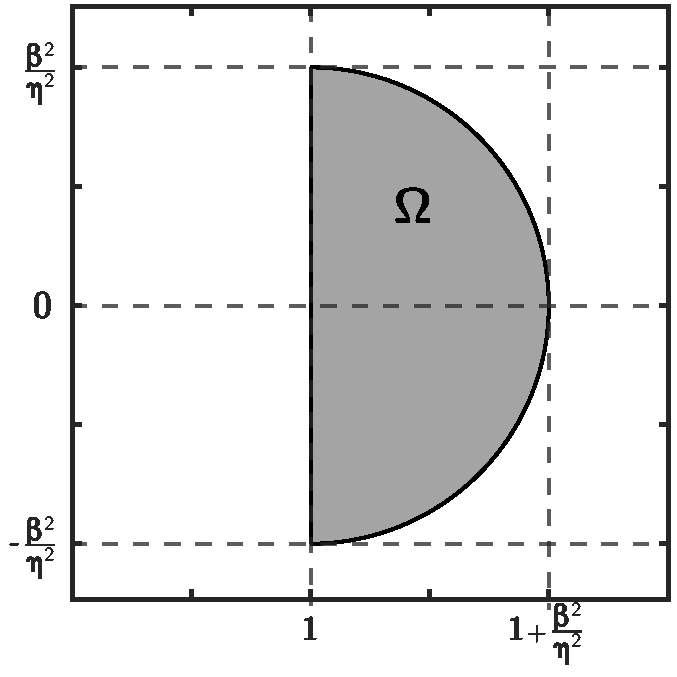
\includegraphics[width = 0.3\textwidth]{./fov_fig.pdf}
% \caption{}
% \label{fig:bound}
% \end{figure}
% %

% However, $\eta$ is probably not the best constant to use. For SPD matrices, 
% somebody proved that using a constant $k := \sqrt{\eta^2+\beta^2}$ and
% preconditioner
% %
% \begin{align*}
% P_k := (k I - \mathcal{L})^{-2}
% \end{align*}
% %
% is a much better choice for $\beta \gg \eta$. I am trying to figure out if
% anything similar can be said for the FOV (or other more general types of
% analysis/operator).

% Note that for real $k>0$, $W\left[\left(I - \tfrac{1}{k}\mathcal{L}\right)^{-1}\right]$ and
% $W\left[\left(I - \tfrac{1}{k}\mathcal{L}\right)^{-2}\right]$ are contained in
% the positive half unit circle. Now consider the more general preconditioning
% %
% \begin{align}\nonumber
% (kI - \mathcal{L})^{-2}\Big[(nI - \mathcal{L})^2 + \beta^2 I\Big] 
% 	& = (kI - \mathcal{L})^{-2}\Big[(\eta-k)I + (kI - \mathcal{L}))^2 + \beta^2 I\Big] \\
% & = (kI - \mathcal{L})^{-2}\Big[(k-\eta)^2I - 2(k-\eta)(kI - \mathcal{L}) + (kI - \mathcal{L})^2 + \beta^2 I\Big] \nonumber\\
% & = I - 2(k-\eta)(kI - \mathcal{L})^{-1} + (\beta^2 + (k-\eta)^2)(kI - \mathcal{L})^{-2} \nonumber\\
% & = I - 2\frac{k-\eta}{k}\left(I - \tfrac{1}{k}\mathcal{L}\right)^{-1} + \frac{\beta^2 + (k-\eta)^2}{k^2}
% 	\left(I - \tfrac{1}{k}\mathcal{L}\right)^{-2}.\label{eq:gen0}
% \end{align}
% %
% Note that we have a quadratic polynomial in $\left(I - \tfrac{1}{k}\mathcal{L}\right)^{-1}$.
% Let $\alpha$ denote the inverse of the roots of the corresponding polynomial.
% Then \eqref{eq:gen1} can be expressed in factored form as
% %
% \begin{align*}
% (kI - \mathcal{L})^{-2}\Big[(nI - \mathcal{L})^2 + \beta^2 I\Big] 
% 	& = \Big[I - \overline{\alpha}\left(I - \tfrac{1}{k}\mathcal{L}\right)^{-1}\Big]
% 	\Big[I - \alpha\left(I - \tfrac{1}{k}\mathcal{L}\right)^{-1}\Big],
% \end{align*}
% %
% where $\alpha + \overline{\alpha} = 2\tfrac{k-\eta}{k}$ and $\alpha\overline{\alpha}
% = \tfrac{\beta^2 + (k-\eta)^2}{k^2}$. For ease of notation, let us denote
% $\mathcal{P} := \left(I - \tfrac{1}{k}\mathcal{L}\right)^{-1}$.
% {\color{blue}
% We are now interested in the field of values of 
% %
% \begin{align*}
% \mathcal{Z} := (I - \overline{\alpha}\mathcal{P})(I - {\alpha}\mathcal{P}).
% \end{align*}
% %
% where $W(\mathcal{P})$ is contained in the positive half of the unit circle.
% This seems like a nice structure and operator, but I'm stuck. I've tried the
% standard symmetric and skew symmetric splittings. The symmetric works okay for
% an opper bound, but I cannot get a lower bound $> 0$. This is all related to
% \eqref{eq:gen0}, in particular how $\langle \mathcal{P}\mathbf{x},\mathbf{x}\rangle$
% and $\langle \mathcal{P}^2\mathbf{x},\mathbf{x}\rangle$ relate? In general I know
% the FOV of $A$ and $A^2$ don't necessarily relate, but there's a lot of nice
% structure here, and numerical results make $k = \sqrt{\eta^2+\beta^2}$ seem
% optimal for very nonsymmetric advective matrices as well.
% }



\end{document}




% ------------------------------------------------------------------- %
% ------------------------------ WRONG ------------------------------
% ------------------------------------------------------------------- %
% \subsubsection{SPD operators}

% Suppose $\widehat{\mathcal{L}}$ is symmetric negative definite and, thus, has an orthogonal
% basis of eigenvectors, and consider the conditioning of \eqref{eq:gamma0}. Assume that the
% eigenvalues of $( I- \tfrac{1}{\eta}\widehat{\mathcal{L}})^{-1} \subset (0,1)$, and are
% somewhat dense in this interval. This is to be expected for parabolic problems, where the
% eigenvalues of $-\widehat{\mathcal{L}}$ range from $\sim \delta t$ to $\sim \delta t/h^2$,
% which typically corresponds to $\sim(0,\infty)$ as $h,\delta t\to 0$.

% Note that \eqref{eq:gamma0} is a quadratic polynomial in an SPD operator, and the
% eigenvalues of \eqref{eq:gamma0} are then a quadratic function $P(\lambda)$ of the
% eigenvalues $\{\lambda\}$ of $\widehat{\mathcal{L}}$, where
% %
% \begin{align}\label{eq:quadratic}
% P(\lambda,\gamma) &:= \frac{\beta^2}{\gamma\eta}\lambda^2 - \frac{\gamma - \eta}{\gamma}\lambda + 1.
% \end{align}
% %
% Assume that we choose $\gamma$ such that \eqref{eq:gamma0} is also SPD (choosing otherwise
% would be a poor choice in terms of conditioning). Then the condition number of
% \eqref{eq:gamma0} is given by
% %
% \begin{align}\label{eq:cond0}
% \textnormal{cond}\left((\gamma I- \widehat{\mathcal{L}})^{-1}S\right) & =
% 	\frac{\lambda_{\max}\left((\gamma I- \widehat{\mathcal{L}})^{-1}S\right)}
% 		{\lambda_{\min}\left((\gamma I- \widehat{\mathcal{L}})^{-1}S\right)}.
% \end{align}
% %
% Again assuming that eigenvalues $\lambda\in\sigma\left(\widehat{\mathcal{L}}\right)$ take
% on values $\lambda\in(0,1)$, the condition number \eqref{eq:cond0} can be expressed
% precisely as $h,\delta t\to 0$ via
% %
% \begin{align}\label{eq:cond1}
% \textnormal{cond}\left((\gamma I- \widehat{\mathcal{L}})^{-1}S\right) & =
% 	\frac{\max_{x\in(0,1)} P(x,\gamma)}{\min_{y\in(0,1)} P(y,\gamma)}.
% \end{align}
% %
% With this closed form, it is natural to pose a minimization problem to find the
% optimal $\gamma$ in terms of minimizing the condition number \eqref{eq:cond0}.
% We make the assumption that $\eta \leq \gamma \leq \eta^2+\beta^2$, and consider
% the problem
% %
% \begin{align*}
% \gamma_* & = \textnormal{argmin}_{\gamma \geq \eta}
% 	\frac{\max_{x\in(0,1)} P(x,\gamma)}{\min_{y\in(0,1)} P(y,\gamma)}.
% \end{align*}
% %

% For $\gamma > 0$, $P(\lambda,\gamma)$ is concave up in $\lambda$, and thus
% the maximum over a closed interval $[0,1]$ will be obtained at one of the
% end points,
% %
% \begin{align*}
% P(0) = 1, \hspace{5ex} P(1) = \frac{\eta^2+\beta^2}{\eta\gamma}.
% \end{align*}
% %
% For the maximum eigenvalue, this yields
% %
% \begin{align}\label{eq:max0}
% \lambda_{\max} & = \begin{cases} 
% 	\frac{\eta^2+\beta^2}{\gamma\eta} & \gamma\leq \frac{\eta^2+\beta^2}{\eta}, \\
% 	1 & \gamma > \frac{\eta^2+\beta^2}{\eta}.
% 	\end{cases}
% \end{align}
% %
% If there is a critical point within the interval $(0,1)$, the minimum
% will be obtained at this critical point, otherwise it will be obtained
% at the other endpoint (i.e., not where the maximum is obtained). Solving
% for $\tfrac{\partial P(\lambda,\gamma)}{\lambda}$ and setting equal to
% zero, we have a root
% %
% \begin{align*}
% \lambda_0 := \frac{\eta(\gamma-\eta)}{ 2\beta^2} \geq 0, \hspace{5ex}
% P(\lambda_0,\gamma) & = 1 - \frac{\eta(\gamma-\eta)^2}{4\beta^2\gamma},
% \end{align*}
% %
% which satisfies $\lambda_0<1$ when $\gamma < \tfrac{2\beta^2+\eta^2}{\eta}$.
% If we suppose $\lambda_0<1$, we have 
% %
% \begin{align}\label{eq:min0}
% \lambda_{\min} & = P(\lambda_0,\gamma) = 1 - \frac{\eta(\gamma-\eta)^2}{4\beta^2\gamma}.
% \end{align}
% %
% For $\gamma \geq \tfrac{\eta^2+2\beta^2}{\eta} > \tfrac{\eta^2+\beta^2}{\eta}$,
% from \eqref{eq:max0}, we have $\lambda_{\min} = \frac{\eta^2+\beta^2}{\gamma\eta}$.
% Altogether, we have the condition number as a continuous function of $\gamma$,
% %
% \begin{align}\label{eq:cases}
% \textnormal{cond}\left((\gamma I- \widehat{\mathcal{L}})^{-1}S\right) & =
% % 	\begin{cases}
% % 		\frac{\frac{\eta^2+\beta^2}{\gamma\eta}}{1 - \frac{\eta(\gamma-\eta)^2}{4\beta^2\gamma}}
% % 			& \gamma\leq \frac{\eta^2+\beta^2}{\eta}, \\
% % 		\frac{1}{1 - \frac{\eta(\gamma-\eta)^2}{4\beta^2\gamma}}
% % 			& \frac{\eta^2+\beta^2}{\eta} \leq \gamma\leq \frac{\eta^2+2\beta^2}{\eta}, \\
% % 		\frac{1}{\frac{\eta^2+\beta^2}{\gamma\eta}}
% % 			& \frac{\eta^2+2\beta^2}{\eta} \leq \gamma.
% % 	\end{cases}
% % \\ & = \textnormal{argmin}_{\gamma \in[\eta,\eta^2+\beta^2]} 
% 	\begin{cases}
% 		\frac{4\beta^2(\eta^2+\beta^2)}{4\beta^2\gamma\eta - \eta^2(\gamma-\eta)^2}
% 			& \eta \leq \gamma< \frac{\eta^2+\beta^2}{\eta}, \\
% 		\frac{4\beta^2\gamma}{4\beta^2\gamma - \eta(\gamma-\eta)^2}
% 			& \frac{\eta^2+\beta^2}{\eta} \leq \gamma < \frac{\eta^2+2\beta^2}{\eta}, \\
% 		\frac{\gamma\eta}{\eta^2+\beta^2}
% 			& \frac{\eta^2+2\beta^2}{\eta} \leq \gamma.
% 	\end{cases}
% \end{align}
% %
% To proceed with the proof, we consider each of these cases individually.\\
% \\
% \underline{$\mathbf{\frac{\boldsymbol{\eta}^2+2\boldsymbol{\beta}^2}{\boldsymbol{\eta}}
% 	\leq \boldsymbol{\gamma}:}$}
% This is the simplest case. Simply note that for $0<\eta\leq \gamma$,
% %
% \begin{align*}
% \frac{\partial}{\partial\gamma} \left[\frac{\gamma\eta}{\eta^2+\beta^2}\right] = 
% 	\frac{\eta}{\eta^2+\beta^2} > 0,
% \end{align*}
% %
% and thus the minimum value for $\gamma \geq \frac{\eta^2+2\beta^2}{\eta}$ is
% obtained at the lower point of the interval, $\gamma = \frac{\eta^2+2\beta^2}{\eta}$.\\
% \\
% \underline{$\mathbf{\frac{\boldsymbol{\eta}^2+\boldsymbol{\beta}^2}{\boldsymbol{\eta}} \leq
% 	\boldsymbol{\gamma} < \frac{\boldsymbol{\eta}^2+2\boldsymbol{\beta}^2}{\boldsymbol{\eta}}}$:}
% Taking the derivative with respect to $\gamma$ from the appropriate equation in
% \eqref{eq:cases}, we get nice cancellation to arrive at
% %
% \begin{align*}
% \frac{\partial}{\partial\gamma} \left[\frac{4\beta^2\gamma}{4\beta^2\gamma - \eta(\gamma-\eta)^2}\right] 
% 	& = 4\beta^2\eta \frac{\gamma^2 - \eta^2}{\left(4\beta^2\gamma - \eta(\gamma-\eta)^2\right)^2}
% 	> 0.
% \end{align*}
% %
% As in the previous case, this yields the minimum value for $\gamma \in\left[\tfrac{\eta^2+\beta^2}{\eta} ,
% \tfrac{\eta^2+2\beta^2}{\eta}\right]$ is obtained at the lower point of the interval,
% $\gamma = \frac{\eta^2+\beta^2}{\eta}$.\\
% \\
% \underline{$\mathbf{\boldsymbol{\eta} \leq \boldsymbol{\gamma}} <
% 	\frac{\boldsymbol{\eta}^2+\boldsymbol{\beta}^2}{\boldsymbol{\eta}}:$}
% Again taking the derivative with respect to $\gamma$ yields
% %
% \begin{align}\label{eq:deriv_gam}
% \frac{\partial}{\partial\gamma} \left[\frac{4\beta^2(\eta^2+\beta^2)}{4\beta^2\gamma\eta
% 	- \eta^2(\gamma-\eta)^2}\right] & =
% 	\frac{4\beta^2(\eta^2+\beta^2)}{\left(4\beta^2\gamma\eta - \eta^2(\gamma-\eta)^2\right)^2}
% 	\left(2\eta^2\gamma - 4\beta^2\eta - 2\eta^3 \right).
% \end{align}
% %
% Note that the sign (and root) of \eqref{eq:deriv_gam} is fully determined by 
% the term on the right, $(2\eta^2\gamma - 4\beta^2\eta - 2\eta^3 )$.
% Setting equal to zero and solving, we have a root at
% %
% \begin{align*}
% \gamma_0 := \frac{2\beta^2 + \eta^2}{\eta} > \frac{\beta^2+\eta^2}{\eta},
% \end{align*}
% %
% where \eqref{eq:deriv_gam} is $<0$ for $\gamma < \gamma_0$. Thus,
% \eqref{eq:deriv_gam} is $<0$ for all $\gamma \in[\eta,\tfrac{\eta^2+\beta^2}{\eta}]$,
% and the minimum value of the function is obtained at the upper end of the interval,
% $\gamma = \frac{\eta^2+\beta^2}{\eta}$.

% Combining the above cases, we have
% %
% \begin{align}\label{eq:gamma_opt}
% \gamma_* & := \frac{\eta^2+\beta^2}{\eta}.
% \end{align}
% %
% with condition number
% %
% \begin{align}\label{eq:opt_cond}
% \textnormal{cond}\left((\gamma_* I- \widehat{\mathcal{L}})^{-1}S\right) & =
% 	1 + \frac{\beta^2}{3\beta^2 + 4\eta^2},
% \end{align}
% %
% whereas using $\eta$ instead of $\gamma_*$ yields condition number
% $1 + \tfrac{\beta^2}{\eta^2}$ \eqref{eq:cases}. Interestingly, if we look at
% the product of the two constants, $\eta\gamma_* = \eta^2+\beta^2$, we have
% the same as when we use a single constant twice in \eqref{eq:gamma_opt0},
% $\gamma_\times^2 = (\sqrt{\eta^2+\beta^2})^2 = \eta^2+\beta^2$.



